\documentclass{article}

\usepackage{ctex}
\usepackage{graphicx}
\usepackage{float}
\usepackage{datetime}
\usepackage{amssymb}
\usepackage{setspace}
\usepackage{amsmath}
\usepackage{geometry}
\usepackage{tikz}
\usetikzlibrary{positioning} %为了实现相对位置的设定
\usepackage{xcolor} %为了实现不同的颜色

\geometry{left=3.0cm,right=2.0cm,top=2.5cm,bottom=2.5cm}
\title{离散数学作业 Problem Set 5}
\renewcommand{\baselinestretch}{1.5} %调整行间距

\author{201830099 周义植}
\date{\today}

\begin{document}
\maketitle
\section*{Problem 1}
证明:(也可以用数学归纳法来做)

对任意$a\in A$,因为R是集合A上的自反关系,所以$(a,a)\in R$,令$t_{1},t_{2}\cdots t_{n-1} = a,$则$(a,t_{1}),(t_{1},t_{2}),\cdots (t_{n-1},a)\in R^{n}$,所以$(a,a)\in R^{n}$,所以$R^{n}$是自反的。

\section*{Problem 2}
$r(R) = R\cup I_{A} = {(===a,a),(b,b),(c,c),(a,b),(b,c)}$

$s(R) = R\cup R^{-1} = {(a,a),(a,b),(b,a),(b,c),(c,b),(c,c)}$

$R^{2} = \{(a,a),(a,b),(a,c),(b,c),(c,c)\}$

$R^{3} = \{(a,a),(a,b),(a,c),(b,c),(c,c)\}$

$t(R) = R\cup R^{2}\cup R^{3} = \{(a,a),(a,b),(a,c),(b,c),(c,c)\}$

\section*{Problem 3}
证明:


自反:对任意正整数对$(a,b),a+b=b+a\therefore ((a,b),(b,a))\in R$

传递:对任意$((a,b),(c,d)),((c,d),(e,f))\in R,$可得出$a+d=b+c,c+f=d+e,$两式子左右相加,有$a+f=b+e,\therefore ((a,b),(e,f))\in R$

对称:对任意$((a,b),(c,d))\in R,$可知$a+d=b+c,\therefore c+b=d+a,((c,d),(a,b))\in R$

综上,关系R为等价关系。
\section*{Problem 4}
证明:

自反:对任意串$x$,其前三位就是自己的前三位,所以$xRx$

传递:对任意$xRy,yRz$,x的前三位等于y的前三位,y的前三位等于z的前三位,因此x的前三位等于z的前三位,所以$xRz$

对称:对任意$xRy$,x的前三位等于y的前三位,y的前三位也等于x的前三位,因此$yRx$

综上,关系R为等价关系。
\section*{Problem 5}
a)\{1\},\{2\},\{3\},\{4\}

b)\{1,2\},\{1,3,4\},\{2,3,4\}

c)不存在。

d)不存在。

e)\{2,4\},\{2,3,4\}

f)\{2,4\}

g)\{3\},\{4\},\{3,4\}

h)\{3,4\}

\section*{Problem 6}
a)是

b)是

c)是

\section*{Problem 7}

证明:
(这里首先要证明是偏序关系)

令X=$
\begin{bmatrix}
    0&0\\
    0&0
\end{bmatrix}$,
Y=$
\begin{bmatrix}
    1&1\\
    1&1
\end{bmatrix}$
\\[10pt]
则对任意$M\in A:XRM , MRY$,所以$X,Y$为$(A,R)$的最小、最大元,因此对任意$M,N\in A,$从最大元逐步向下找,一定存在上确界。同理也一定存在下确界。因此$(A,R)$为格。
\section*{Problem 8}

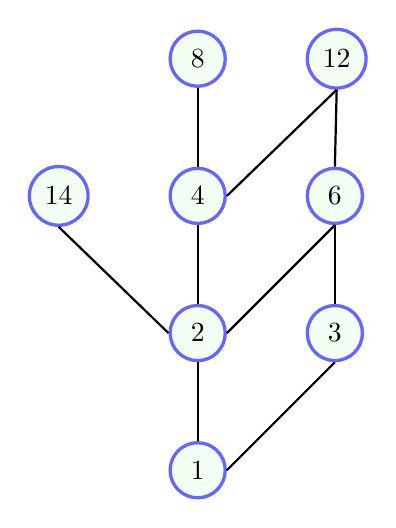
\begin{tikzpicture}[
% 设定样式
roundnode/.style={circle, draw=blue!60, fill=green!5, very thick, minimum size=7mm},
squarednode/.style={rectangle, draw=red!60, fill=red!5, very thick, minimum size=5mm},
]
%定义节点:Nodes
\node[roundnode]      (a1)                              {8};
\node[roundnode]        (a2)       [right=of a1] {12};
\node[roundnode]      (b1)       [below=of a1] {4};
\node[roundnode] (b0) [left=of b1] {14};
\node[roundnode] (b2) [right=of b1] {6};
\node[roundnode] (c1) [below=of b1] {2};
\node[roundnode] (c2) [right=of c1] {3};
\node[roundnode] (d1) [below=of c1] {1};

%Lines
\draw[thick,-] (a1.south) -- (b1.north);
\draw[thick,-] (a2.south) -- (b1.east);
\draw[thick,-] (a2.south) -- (b2.north);
\draw[thick,-] (b1.south) -- (c1.north);
\draw[thick,-] (b2.south) -- (c2.north);
\draw[thick,-] (c1.south) -- (d1.north);
\draw[thick,-] (b0.south) -- (c1.west);
\draw[thick,-] (b2.south) -- (c1.east);
\draw[thick,-] (c2.south) -- (d1.east);
% \draw[thick,->] (rightsquare.south) .. controls +(down:7mm) and +(right:7mm) .. (lowercircle.east);

\end{tikzpicture}

极大元:4,6;

极小元:2,3

最大元:不存在

最小元:不存在。

最小上界:12

最大下界:1
\section*{Problem 9}
(1)$R = \{(1,2),(1,1),(2,1),(2,2),(2,3),(3,3),(3,2),(1,3),(3,1),(4,4),(5,5),(4,5),(5,4)\}$

(2) 
\begin{equation}\label{Eq:matrix1}
    \bordermatrix{%
           & 1      & 2    &3     &4 &5\cr
    1    & 1         & 1       &1     & 0 &0 \cr
    2   & 1        & 1      &1    & 0   &0 \cr
    3 & 1   &1  &1   &0  &0 \cr
    4  & 0         & 0     &0    &1     &1 \cr
    5 & 0          &0        &0         &1     &1
    },
    \end{equation}
\clearpage
(3)

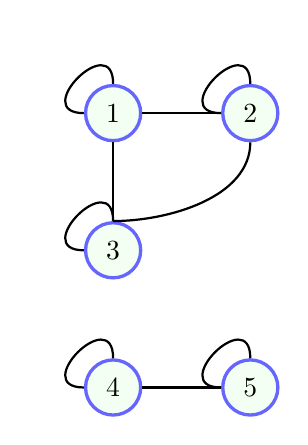
\begin{tikzpicture}[
    % 设定样式
    roundnode/.style={circle, draw=blue!60, fill=green!5, very thick, minimum size=7mm},
    squarednode/.style={rectangle, draw=red!60, fill=red!5, very thick, minimum size=5mm},
    ]
    %定义节点:Nodes
    \node[roundnode]      (a1)                              {1};
    \node[roundnode]        (a2)       [right=of a1] {2};
    \node[roundnode]      (a3)       [below=of a1] {3};
    \node[roundnode] (b1) [below=of a3] {4};
    \node[roundnode] (b2) [right=of b1] {5};
  
    
    %Lines
    \draw[thick,-] (a1.south) -- (a3.north);
    \draw[thick,-] (a1.east) -- (a2.west);
    \draw[thick,-] (a2.south) .. controls +(down:7mm) and +(right:7mm) .. (a3.north);
    \draw[thick,-] (b1.east) -- (b2.west);
    \draw[thick,-] (a1.north) .. controls +(up:7mm) and +(left:7mm) .. (a1.west);
    \draw[thick,-] (a2.north) .. controls +(up:7mm) and +(left:7mm) .. (a2.west);
    \draw[thick,-] (a3.north) .. controls +(up:7mm) and +(left:7mm) .. (a3.west);
    \draw[thick,-] (b1.north) .. controls +(up:7mm) and +(left:7mm) .. (b1.west);
    \draw[thick,-] (b2.north) .. controls +(up:7mm) and +(left:7mm) .. (b2.west);
    % \draw[thick,->] (rightsquare.south) .. controls +(down:7mm) and +(right:7mm) .. (lowercircle.east);
    
    \end{tikzpicture}

\section*{Problem 10}
分类讨论:

1+1+1+1 : 1

2+1+1 : $\binom{4}{2} $

2+2 : $\binom{4}{2}/2 $

3+1: $\binom{4}{3} $

4: $1$

所以共有$1+\binom{4}{1} +\binom{4}{2}/2 + \binom{4}{2} + 1 = 15 $种。
\end{document}